%%%%%%%%%%%%%%%%%%%%%%%%%%%%%%%%%%%%%%%%%
%
% This template was modified by Gustavo Pantuza as in
% http://github.com/pantuza/vitex
%
% Plasmati Graduate CV
% LaTeX Template
% Version 1.0 (24/3/13)
%
% This template has been downloaded from:
% http://www.LaTeXTemplates.com
%
% Original author:
% Alessandro Plasmati (alessandro.plasmati@gmail.com)
%
% License:
% CC BY-NC-SA 3.0 (http://creativecommons.org/licenses/by-nc-sa/3.0/)
%
% Important note:
% This template needs to be compiled with XeLaTeX.
% The main document font is called Fontin and can be downloaded for free
% from here: http://www.exljbris.com/fontin.html
%
%%%%%%%%%%%%%%%%%%%%%%%%%%%%%%%%%%%%%%%%%




%----------------------------------------------------------------------------------------
%	PACKAGES AND OTHER DOCUMENT CONFIGURATIONS
%----------------------------------------------------------------------------------------

\documentclass[a4paper,10pt]{article} % Default font size and paper size

\usepackage{fontspec} % For loading fonts
\defaultfontfeatures{Mapping=tex-text}
\setmainfont[SmallCapsFont = Fontin SmallCaps]{Fontin} % Main document font

\usepackage{xunicode,xltxtra,url,parskip} % Formatting packages

\usepackage[usenames,dvipsnames]{xcolor} % Required for specifying custom colors

\usepackage[big]{layaureo} % Margin formatting of the A4 page, an alternative to layaureo can be \usepackage{fullpage}
% To reduce the height of the top margin uncomment: \addtolength{\voffset}{-1.3cm}

\usepackage{hyperref} % Required for adding links	and customizing them
\definecolor{linkcolour}{rgb}{0,0.2,0.6} % Link color
\hypersetup{colorlinks,breaklinks,urlcolor=linkcolour,linkcolor=linkcolour} % Set link colors throughout the document

\usepackage{titlesec} % Used to customize the \section command

\usepackage{longtable} % Used for footnotes inside tables
\usepackage{makecell} % Allow to break lines inside one cell

\usepackage{floatrow} % Image and table side by side
% Table float box with bottom caption, box width adjusted to content
\newfloatcommand{capbtabbox}{table}[][\FBwidth]

\titleformat{\section}{\Large\scshape\raggedright}{}{0em}{}[\titlerule] % Text formatting of sections
\titlespacing{\section}{0pt}{3pt}{3pt} % Spacing around sections

\begin{document}

\pagestyle{empty} % Removes page numbering

\font\fb=''[cmr10]'' % Change the font of the \LaTeX command under the skills section




%----------------------------------------------------------------------------------------
%	NAME AND CONTACT INFORMATION
%----------------------------------------------------------------------------------------

\par{\centering{\Huge Gustavo \textsc{Pantuza}}\bigskip\par} % Your name

\section{Dados Pessoais}

\begin{figure}[ht]
\begin{floatrow}

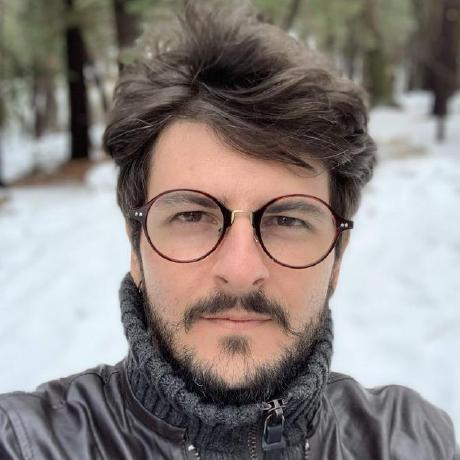
\includegraphics[width=.2\textwidth]{thumb.jpg}

\capbtabbox{%
\begin{tabular}{rl}
\textsc{Nascimento:} & 12 de Outubro de 1989 \\
\textsc{Endereço:} & Belo Horizonte - MG \\
\textsc{Telefone:} & +55 31 9 8367 2657 \\
\textsc{email:} & \href{mailto:gustavopantuza@gmail.com}{gustavopantuza@gmail.com} \\
\textsc{Pesquisa:} & \href{https://scholar.google.com/citations?user=V6xqvdgAAAAJ}{Perfil no Google Scholar} \\
\textsc{Blog:} & \href{https://blog.pantuza.com}{https://blog.pantuza.com} \\
\textsc{Github:} & \href{https://github.com/pantuza}{https://github.com/pantuza}
\end{tabular}
}

\end{floatrow}
\end{figure}




%----------------------------------------------------------------------------------------
%	WORK EXPERIENCE
%----------------------------------------------------------------------------------------

\section{Experiências Profissionais}

\begin{longtable}{r|p{11cm}}

\textsc{Jan 2025 - Atual} & \emph{\bf Doutorando em Ciência da Computação na UFMG}, \\
& \footnotesize{
  Sou doutorando na Universidade Federal de Minas Gerais (UFMG) no
  departamento de Ciência da Computação. Minha pesquisa é focada na interseção dos
  tópicos: Sistemas Distribuídos e Observabilidade. Estou trabalhando em um projeto
  que visa melhorar a resiliência de aplicações observando dados de Profiling de 
  redes massivamente distribuídas.
  } \\
\multicolumn{2}{c}{} \\

\textsc{Out 2023 - Atual} & \emph{\bf Staff Software engineer na Doximity}, \\
& \footnotesize{
  Trabalho na equipe de Site Reliability Engineering (SRE) e lidero a iniciativa de observabilidade através
  da adoção do protocolo Open Telemetry e seu ecossistema. Eu projetei e implementei pipelines de telemetria
  para coletar, processar e armazenar logs, métricas e rastros. Um dos aspectos críticos deste projeto foi
  migrar de soluções de observabilidade anteriores para uma nova sem incidentes em produção e ainda reduzindo
  custos. Colaborar com várias equipes, executar sessões de compartilhamento de conhecimento e escrever
  documentação foram aspectos essenciais do meu trabalho. Otimizações como amostragem, retenção de dados e 
  dimensionamento correto da infraestrutura também foram desafios que venho resolvendo.
  } \\
\multicolumn{2}{c}{} \\

\textsc{Jul 2023 - Atual} & \emph{\bf Consultor em Ciência da Computação}, \\
& \footnotesize{
  Realizo treinamentos, serviços de consultoria para empresas e desenvolvedores
  na área de Observabilidade, Sistemas Distribuídos e Computação em Nuvem. Ajuda
  empresas a adotar e obter uma transição suave para tecnologias como Open Telemetry,
  Kubernetes e Service Meshes.
  } \\
\multicolumn{2}{c}{} \\

\textsc{Out 2021 - Out 2023} & \emph{\bf Staff Software engineer na VTEX}, \\
& \footnotesize{
    Primeiro, trabalhei revisando a arquitetura das equipes para melhorar
    a resiliência em relação ao design de sistemas distribuídos. Depois, ajudei
    a projetar uma equipe de Engenharia de Tráfego sendo responsável pela implementação de CDNs,
    API Gateways, soluções de cache e balanceamento de carga. Por fim, trabalhei na
    equipe de Observabilidade projetando uma solução de longo prazo para logs, métricas e
    rastreamentos de forma que a VTEX pudesse depurar, solucionar problemas e fazer descobertas
    em seu ambiente de produção. Uma das minhas principais funções era colaborar entre equipes.
    Este projeto rendeu uma apresentação na KubeCon 2023 (ver sessão palestras).
  } \\
\multicolumn{2}{c}{} \\

\textsc{Abr 2019 - Out 2021} & \emph{\bf Software engineer IV na GoDaddy}, \\
& \footnotesize{
    Eu era responsável por colaborar com outras equipes para projetar
    a arquitetura de segurança de sites da GoDaddy em escala global e como 
    reutilizar o código em nossos serviços distribuídos.
    Como engenheiro de software, trabalhei escrevendo um serviço para escanear
    80 milhões de domínios da Internet diariamente. O serviço procurava vulnerabilidades de
    segurança, URLs na lista de bloqueio, assinaturas maliciosas conhecidas,
    problemas de TLS, versões desatualizadas de softwares, registros de DNSs e muito mais.
    Trabalhei escrevendo código em Golang, C lang e Kubernetes para atingir a
    escala necessária diariamente. Além disso, como engenheiro de software, fui responsável 
    por codificar, testar, monitorar e gerenciar o ciclo de vida desta aplicação.
    Trabalhei remotamente com uma equipe distribuída em vários países. } \\
\multicolumn{2}{c}{} \\

\textsc{Mar 2015 - Mar 2019} & \emph{\bf Engenheiro de software sênior na Globo.com}, \\
& \footnotesize{Trabalho em um projeto de software livre escrito em Python
    chamado \href{https://github.com/globocom/GloboNetworkAPI}{Network API}.
    É um serviço de \emph{cloud} que tem visão global sobre a infraestrutura
    de redes. Tem controle sobre cada IP alocado, recurso utilizado e
    provisionamento de equipamentos. Na Globo.com é utilizado para controlar
    todo o \emph{datacenter}. No ambiente interno de \emph{cloud} integra-se
    com CloudStack, Xen, Tsuru, DBaaS entre outros projetos privados em nuvem.

    Anteriormente, trabalhei no Globo Core, um time responsável pela aplicação
    que faz a entrega final de páginas Web (CDA - \emph{Content delivery
    application}) e também no ciclo de vida do conteúdo (CMA - \emph{Content
    management application}). O primeiro deve ser o mais rápido possível e
    é utilizado nos principais portais da Globo.com como G1, Gshow e Globo
    Esporte. O segundo é uma plataforma Web onde jornalistas e editores
    escrevem o conteúdo.} \\
\multicolumn{2}{c}{} \\

\textsc{Fev 2012 - Dez 2014} & \emph{\bf Mestre em Ciência da Computação pela
    Universidade Federal de Minas Gerais (UFMG). Pesquisador em
Redes e Sistemas Distribuídos}, \\
& \footnotesize{Como pesquisador pelo Conselho Nacional de Desenvolvimento
    Científico e Tecnológico (CNPq) eu escrevi a seguinte dissertação: Grafos
    como uma primitiva do plano de controle para análise e gerenciamento de
    Redes Definidas por Software.

    Durante esse período cursei matérias como Projeto e análise de algoritmos,
    processamento de dados massivos, Algoritmos distribuídos, Engenharia de
    aplicações em rede, Sistemas Operacionais, Redes inteligentes e Padrões de
    programação paralela.

    Dentro do laboratório WiNET, escrevi um programa balanceador de carga IP
    através do controlador SDN POX. Além disso, criei um módulo em grafos que
    mantém uma visão global da topologia de redes e escuta eventos de entrada
    e saída de máquinas e enlaces na rede. O grafo serve como uma ferramenta de
    gerenciamento.} \\
\multicolumn{2}{c}{} \\

\textsc{Set 2012 - Jun 2013} & \emph{\bf Engenheiro de Software e Administrador
de Sistemas na Latitude 14} \\
& \footnotesize{Trabalhei com uma equipe dedicada de 7 pessoas em um portal de
    música independente. Nesse projeto privado para a Telefonica Brasil S/A
    (Vivo) participei da implantação de servidores através do AWS EC2, Cloud
    Front, RDS, S3, Route 53 com aplicações em Django e Postgres. Como time,
    criamos, mantivemos e evoluímos o projeto. Participei de muitas reuniões
    com investidores para discutir futuro e definir metas incrementais.} \\
\multicolumn{2}{c}{} \\

%------------------------------------------------

\textsc{Ago 2010-Set 2012} & \emph{\bf Engenheiro de Software na
Studio Sol Comunicação Digital}  \\
& \footnotesize{Criei APIs e aplicações Web com Python/Django, MySQL,
    Javascript, html/css e PHP para 3 produtos: Letras, Cifra-club e PalcoMP3.
    O Letras tem 30 milhões pageviews/dia. Cifra-club 10 milhões/dia. O
    aplicativo do PalcoMP3 tem 100 milhões de \emph{downloads} no Google play.
    Administrei também projetos como Lucene Solr, Nginx, MongoDB, Redis, uWSGI
    em infraestrutura de servidores dedicados
}\\
\multicolumn{2}{c}{} \\

%------------------------------------------------

\textsc{Jan 2009 - Ago 2010} & \emph{\bf Analista de Teste de Software
na Totvs S.A} \\
& \footnotesize{Participei do desenho de processos de testes dentro de
metodologias interativo/incremental com foco em gerência de configuração,
automação de \emph{build} e documentação.}

\end{longtable}

\footnotetext{Mais experiências descritas no
\href{https://www.linkedin.com/in/gustavo-pantuza-46089825/}{perfil do Linkedin}} 


%----------------------------------------------------------------------------------------
%	EDUCATION
%----------------------------------------------------------------------------------------

\section{Formação}

\begin{tabular}{rl}
\textsc{Dezembro} 2014 & Mestrado em Ciência da Computação na área de
\textsc{Redes e Sistemas Distribuídos}
\\ & na (UFMG)
\textbf{Universidade Federal de Minas Gerais} \\
& Dissertação: ``Grafos como uma primitiva do plano de controle para análise e
\\ & gerenciamento de redes definidas por software''
| \small Orientador: Prof. Luiz \textsc{F M Vieira} \\
&\\

%------------------------------------------------

\textsc{Dezembro} 2012& Bacharel em \textsc{Ciência da Computação}
pelo \normalsize\textbf{Centro Universitário de}
\\ & \textbf{Belo Horizonte}, UNIBH \\
& Projeto de Conclusão: ``Monitoramento e cuidado ao Idoso baseado em
\\ & Sistemas Distribuídos e Microcontroladores''
| \small Orientador: Euzébio \textsc{Souza} \\
&\\

%------------------------------------------------

\textsc{Dezembro} 2007 & Técnico em Informática Industrial,
\textbf{Escola Técnica Juscelino Kubitschek}, Ipatinga \\
&\\

%------------------------------------------------

\textsc{Julho} 2007 & Língua Inglesa, \textbf{Uptime Consultants}
\end{tabular}




%----------------------------------------------------------------------------------------
%	SCHOLARSHIPS AND ADDITIONAL INFO
%----------------------------------------------------------------------------------------

\section{Comunidades e Constribuições}

\begin{tabular}{rl}
\textsc{OpenSUSE}  & Membro da Comunidade OpenSUSE \\
\textsc{Python Brasil}  & Membro da Associação Python Brasil \\
\textsc{Mininet}  & Contribuiu adicionando ambientes de simulação de redes
dinâmicas \\
\textsc{FsF} & Membro da Free Software Foundation \\
\textsc{Área31 Hackerspace} & Membro fundador do
\href{http://area31.net.br}{Hackerspace} \\
\textsc{Pox} & Adicionou uma representação em grafos da rede com a
\\ & finalidade de gerenciamento em redes \\
\textsc{Projetos Pessoais} & \href{http://github.com/pantuza}{Projetos}
pessoais em Software Livre \\
\end{tabular}




%----------------------------------------------------------------------------------------
%	LANGUAGES
%----------------------------------------------------------------------------------------

%\section{Languages}

%\begin{tabular}{rl}
%\textsc{English:} & Fluent\\

%\textsc{Italian:} & Mothertongue\\

%\textsc{French:} & Basic Knowledge\\
%\end{tabular}




%----------------------------------------------------------------------------------------
%	Base de conhecimento
%----------------------------------------------------------------------------------------

\section{Base de conhecimento}

\begin{longtable}{rl}
Linguagens: & Go, C++, C, Python, bash, Ruby, javascript, Java, PHP, html/css, {\fb \LaTeX}
\footnote{Esse documento foi gerado utilizando {\fb \LaTeX} e está
disponível como um \href{http://github.com/pantuza/vitex}{projeto}
de Software Livre no Github.} \\
Bancos de Dados: & MySQL, PostgreSQL, MongoDB, Redis \\
Sistemas Operacionais: & OpenSUSE, CentOS, Ubuntu, Fedora, Arch Linux \\
Serviços: & kubernetes, nginx, memcached, Lucene Solr, squid, bind9, uWSGI, Cron \\
Ferramentas de Rede: & nmap, tcpdump, iptraf, iperf \\
Ferramentas de Cloud: & KVM, Docker, LXC, Cloud Stack \\
Ferramentas de Desenvolvimento: & vim, git, gdb, valgrind, POSIX tools \\
Ciência da Computação: & Algoritmos, Redes, Sistemas distribuídos, Sistemas operacionais \\
\end{longtable}


%----------------------------------------------------------------------------------------
%	Publications
%----------------------------------------------------------------------------------------

\section{Publicações}

\begin{longtable}{rl}
    \href{https://ieeexplore.ieee.org/abstract/document/9631262/}{2021 IEEE ISCC}: & \makecell[l]{
    eQUIC gateway: Maximizing QUIC throughput using a gateway service \\ based on eBPF+ XDP} \\
    \href{https://ieeexplore.ieee.org/abstract/document/9631451/}{2021 IEEE ISCC}: & \makecell[l]{
    Danian: tail latency reduction of networking application through \\ an O (1) scheduler} \\

    \href{https://sol.sbc.org.br/livros/index.php/sbc/catalog/view/50/232/469-1}{SBRC 2020}: & \makecell[l]{[pt-BR]
    Serverless Computing: Concepts, applications and challenges} \\
    \href{https://homepages.dcc.ufmg.br/~mmvieira/cc/papers/Erik_Link_balancing.pdf}{[2015]}: & \makecell[l]{Enforcing Link Utilization with Traffic Engineering on SDN} \\
    \href{https://ieeexplore.ieee.org/document/7014202}{CNSN 2014}: & \makecell[l]{Network Management through Graphs in Software Defined Networks} \\
\href{http://www.sbrc2014.ufsc.br/anais/files/wpeif/anaisWPEIF2014.pdf}{SBRC 2014}: & \makecell[l]{[pt-BR] Análise e Gerenciamento de Rede através de Grafos \\
    em Redes Definidas por Software} \\
\href{https://www.dcc.ufmg.br/pos/cursos/defesas/1824M.PDF}{Master thesis}: & \makecell[l]{[pt-BR] Graphs as a primitive of the control plane to network analisys \\
    and management through Software Defined Networking} \\
\end{longtable}


%----------------------------------------------------------------------------------------
%	Talks
%----------------------------------------------------------------------------------------

\section{Palestras}

\begin{longtable}{rl}
\href{https://www.youtube.com/watch?v=aDysORX1zIs}{KubeCon 2023}: & \makecell[l]{Ingesting 6.5 Tb of Telemetry Data Daily Through Open \\ 
  Telemetry Protocol and Collectors \\
\href{https://speakerdeck.com/pantuza/kubecon-europe-2023-ingesting-6-dot-5-tb-of-telemetry-data-daily-through-open-telemetry-protocol-and-collectors}{slides} - \href{https://www.youtube.com/watch?v=aDysORX1zIs}{video}} \\
\href{https://ossna2017.sched.com/speaker/gustavo.pantuza}{Open Source Summit 2017 - LA}: & \makecell[l]{Automating Access Control Lists with OpenDaylight \\
    and OpenVSwitch \\
\href{https://speakerdeck.com/pantuza/automating-access-control-lists-with-opendaylight-and-openvswitch}{slides}} \\
\href{http://fisl18.softwarelivre.org/index.php/en/}{FISL 2018}: & \makecell[l]{Wrapping C libraries into Python Modules \\
\href{https://speakerdeck.com/pantuza/wrapping-c-libraries-into-python-modules}{slides} - \href{https://www.youtube.com/watch?v=g3u1Qw6JcFo}{video}} \\
\href{https://qconsp.com/}{QCON São Paulo}: & \makecell[l]{Resiliência em micro-serviços \\
\href{https://speakerdeck.com/pantuza/resiliencia-em-micro-servicos}{slides} - \href{https://www.youtube.com/watch?v=1-Mr0MJcy00}{video}} \\
Outras Palestras: & \makecell[l]{\href{https://blog.pantuza.com/palestras}{Lista de palestras}} \\
\end{longtable}



%----------------------------------------------------------------------------------------
%	INTERESTS AND ACTIVITIES
%----------------------------------------------------------------------------------------

\section{Atividades e Interesses}
Visite meu site \href{https://pantuza.com}{https://pantuza.com}
e conheça meu código, assim como meu convívio em redes sociais e meus
interesses.
Tenho o hábito de escrever artigos sobre ciência da computação em meu
blog \href{https://blog.pantuza.com}{https://blog.pantuza.com}

%----------------------------------------------------------------------------------------
\end{document}
